\documentclass[12pt]{article}
\usepackage[utf8]{inputenc}
\usepackage{hyperref}
\usepackage{listings}
\usepackage{xcolor}
\usepackage{geometry}
\usepackage{graphicx} % For including graphics

\usepackage{minted} % For advanced code listings

% Define a custom minted style (optional)
\usemintedstyle{colorful} % You can choose from various styles like 'monokai', 'tango', 'colorful', etc.

% Custom color setup
\definecolor{bashtextcolor}{RGB}{0, 0, 0} % Define black color

% Define a new command for inline code using minted
\newcommand{\codeinline}[1]{\mintinline{text}{#1}}

\geometry{a4paper, margin=1in}

\title{Smart Contracts Exercise 03: \\ ERC-20 CTU Token}
\author{}
\date{}

% Define a new command for inline code with a dark background
\newcommand{\codeblack}[1]{%
  \texttt{\colorbox{black!7}{\textcolor{black}{#1}}}%
}

% Define a new command for inline code with a dark background
\newcommand{\codegrey}[1]{%
  \texttt{\colorbox{black!4}{\textcolor{black}{#1}}}%
}

% Define custom colors (optional)
\definecolor{myURLColor}{RGB}{0, 102, 204} % Example: A shade of blue

\hypersetup{
    colorlinks=true,        % Enable colored links
    linkcolor=blue,         % Color for internal links (e.g., \ref, \cite)
    citecolor=blue,         % Color for citations
    filecolor=magenta,      % Color for file links
    urlcolor=myURLColor     % Color for external URLs
}

% Define a style for code listings
\lstdefinestyle{mystyle}{
    backgroundcolor=\color{lightgray!20},   
    commentstyle=\color{green!50!black},
    keywordstyle=\color{blue},
    numberstyle=\tiny\color{gray},
    stringstyle=\color{red},
    basicstyle=\ttfamily\footnotesize,
    breakatwhitespace=false,         
    breaklines=true,                 
    captionpos=b,                    
    keepspaces=true,                 
    numbers=left,                    
    numbersep=5pt,                  
    showspaces=false,                
    showstringspaces=false,
    showtabs=false,                  
    tabsize=2
}

\lstset{style=mystyle}
% Adding package for header and footer
\usepackage{fancyhdr}
\pagestyle{fancy}

% Define header and footer
\fancyhf{} % Clear current settings
\fancyhead[L]{Smart Contracts Exercise 03} % Left header
\fancyhead[R]{\thepage} % Right header with page number

\renewcommand{\headrulewidth}{0.4pt} % Line below header
% \renewcommand{\footrulewidth}{0.4pt} % Line above footer

\begin{document}

\maketitle
\section{Introduction}

Tokens in the Ethereum ecosystem are smart contracts that implement a standardized interface. They are designed to virtually represent certain assets. For example, financial assets such as shares in a company, use as cryptocurrencies (stable coins like USDC, DAI), allow holders to vote on decisions in decentralized projects (e.g., Uniswap - UNI), enable artists to tokenize their works and sell them as unique digital items (NFTs), represent collectibles in games, or are used for digital identity or access to services. Depending on the use case, there are different types of tokens, each serving different purposes. Below are three common types of tokens:

\begin{enumerate}
  \item \textbf{Fungible Tokens}

  Fungible tokens \href{https://ethereum.org/en/developers/docs/standards/tokens/erc-20/}{(\textit{ERC-20 Tokens})} are interchangeable and have exactly the same value. Each unit of a fungible token is identical to another unit. Examples are cryptocurrencies, utility tokens or governance tokens.

    \begin{figure}[h!]
      \centering
      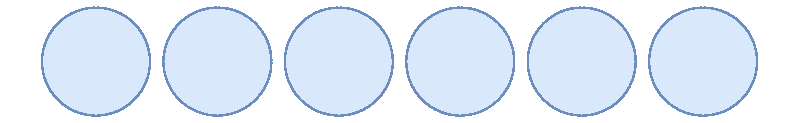
\includegraphics[width=0.5\textwidth]{fungible-tokens.pdf}
      \caption{Fungible Tokens}
      \label{fig:fungible-tokens}
    \end{figure}

    \item \textbf{Non-Fungible Tokens (NFTs)}

    Non-fungible tokens \href{https://ethereum.org/en/developers/docs/standards/tokens/erc-721/}{(\textit{ERC-721 Tokens})} are unique and cannot be exchanged on a one-to-one basis. They are used to represent ownership of unique items such as digital art, collectibles, and real estate. Each token is uniquely identifiable by an ID.

    \begin{figure}[h!]
      \centering
      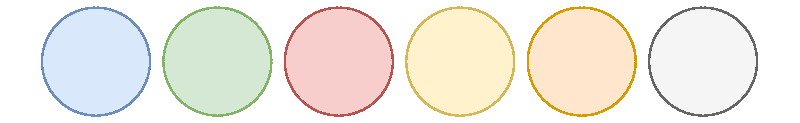
\includegraphics[width=0.5\textwidth]{non-fungible-tokens.pdf}
      \caption{Non-Fungible Tokens}
      \label{fig:non-fungible-tokens}
    \end{figure}

    \item \textbf{Multi-Tokens}

    Multi-tokens \href{https://ethereum.org/en/developers/docs/standards/tokens/erc-1155/}{(\textit{ERC-1155 Tokens})} combine the properties of both fungible and non-fungible tokens. They allow for the creation of multiple token types within a single contract, providing flexibility for various use cases.

    \begin{figure}[h!]
      \centering
      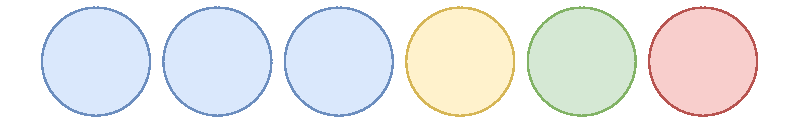
\includegraphics[width=0.5\textwidth]{multi-token.pdf}
      \caption{Multi-Tokens}
      \label{fig:multi-token}
    \end{figure}
  \end{enumerate}

In this exercise, you will create your own ERC-20 token contract according to the specified standard, and then we will attempt to hack this contract together.

\subsection{Prerequisites}

Ensure that you have already installed the following on your system:

\begin{itemize}
    \item \textbf{Node.js} - \url{https://nodejs.org/en/}
    An open-source, cross-platform, back-end JavaScript runtime environment that runs on the V8 engine and executes JavaScript code outside a web browser. 
    \item \textbf{NPM}: Node Package Manager, which comes with Node.js.
\end{itemize}

Open your terminal and run the following commands to verify the installations:

\begin{minted}[bgcolor=gray!5, fontsize=\footnotesize]{bash}
$ node -v
$ npm -v
\end{minted}

Both commands should return the installed version numbers of Node.js and NPM respectively. Node.js provides the runtime environment required to execute JavaScript-based tools like Hardhat, while NPM is used to manage the packages and dependencies needed for development. It is recommended that you use NPM 7 or higher.

\subsection{Project Set Up}

To get started, visit the following \href{https://gitlab.fel.cvut.cz/radovluk/smart-contracts-exercises/-/tree/main/02-Decentralized-Voting-System/task/task-code?ref_type=heads}{GitLab repository} and clone it to your local machine. This repository contains a template in which you will complete this exercise. After you clone the repository start with the following command within your project folder:

\begin{minted}[bgcolor=gray!5, fontsize=\footnotesize]{bash}
  $ npm install
\end{minted}
This will install all the necessary dependencies for the project. Your implementation will be in the file \textit{contracts/Voting.sol}. In this file, there are \#TODO comments where you should implement the required functionality. To fulfill this task you need to pass all the provided tests. You can run the tests with the following command:

\begin{minted}[bgcolor=gray!5, fontsize=\footnotesize]{bash}
  $ npx hardhat test
\end{minted}

There is also a deployment script in the \textit{scripts} folder. You can deploy the contract to the local hardhat network with the following command:
\begin{minted}[bgcolor=gray!5, fontsize=\footnotesize]{bash}
  $ npx hardhat run scripts/deploy.js
\end{minted}

\section{Specification: Voting Contract}

\subsection{Overview}

The \textbf{Voting} contract is a simple implementation of a voting system using Solidity. It allows the contract owner to add candidates, and any address to vote exactly once for a candidate. The contract includes the following functionalities:
\begin{itemize}
    \item The contract owner can add candidates.
    \item Any address can vote exactly once for a candidate.
    \item The contract tracks the number of votes each candidate has received.
    \item The contract tracks whether an address has already voted.
    \item A function to get the total number of candidates.
    \item A function to retrieve a candidate's name and vote count by index.
    \item A function to get the index of the winning candidate.
\end{itemize}

\subsection{Solidity Crash Course}

The \textbf{Voting} contract is designed to facilitate a decentralized voting system. Below are some solidity code snippets that you might find useful for implementing the contract and explanations of the key components.

\subsubsection{State Variables}

\textbf{State variables} are used to store data permanently on the blockchain. They represent the contract's state and can be accessed and modified by the contract's functions.

\begin{minted}[bgcolor=gray!5, fontsize=\footnotesize]{solidity}
  // Address of the contract owner
  address public owner;

  // Dynamic array to store all candidates
  Candidate[] public candidates;

  // Mapping to track whether an address has already voted
  mapping(address => bool) public hasVoted;
\end{minted}

\subsubsection{Structs}

\textbf{Structs} are custom data types that allow you to group related data together. They are useful for organizing complex data structures within the contract.

\begin{minted}[bgcolor=gray!5, fontsize=\footnotesize]{solidity}
  /**
  * @dev Struct to represent a candidate.
  * @param name The name of the candidate.
  * @param voteCount The number of votes the candidate has received.
  */
 struct Candidate {
     string name;
     uint voteCount;
  }
\end{minted}

\subsubsection{Modifiers}

\textbf{Modifiers} are used to change the behavior of functions in a declarative way. They can enforce rules or conditions before executing a function's code.

\begin{minted}[bgcolor=gray!5, fontsize=\footnotesize]{solidity}
  // Modifier to restrict access to the contract owner
  modifier onlyOwner() {
      require(msg.sender == owner, "Only the owner can call this function");
      _; // Continue executing the function
  }

  function addCandidate(string memory _name) public onlyOwner {
    // Only the contract owner can call this function
  }
\end{minted}

\subsubsection{Functions}

\textbf{Functions} define the behavior of the contract. They can read and modify the contract's state, perform computations, and interact with other contracts or external systems.

\subsubsection{Events}

\textbf{Events} are used to log information on the blockchain that can be accessed by off-chain applications. They are essential for tracking contract activities and facilitating interactions with the user interface.

\begin{minted}[bgcolor=gray!5, fontsize=\footnotesize]{solidity}
  /**
  * @dev Event emitted when a vote is cast.
  * @param voter The address of the voter.
  * @param candidateIndex The index of the candidate voted for.
  */
 event Voted(address indexed voter, uint indexed candidateIndex);

 /**
  * @dev Event emitted when a new candidate is added.
  * @param name The name of the candidate to be added.
  */
 event CandidateAdded(string name);
\end{minted}

\subsubsection{Functionality Provided by Solidity}
Here are some useful code snippets you might need:

\begin{minted}[bgcolor=gray!5, fontsize=\footnotesize]{solidity}
// Sender of the transaction
address sender = msg.sender;

// Amount sent with the transaction
uint amount = msg.value;

// Enforcing conditions
require(condition, "Error message");

// Casting arbitrary data to uint
uint number = uint(data);

// Empty address
address emptyAddress = address(0);

// Emit an event
emit EventName(parameters);
\end{minted}


\end{document}
